\chapter{Experiments and results}
\label{chap5:title}

In this chapter we present the test results of the application, which sends WRITE 10 and WRITE SAME 10 commands with different parameters. We made all the tests with WRITE 10 command, when the disks were connected with the enclosure to the controller. But some tests with WRITE SAME 10 command were done with the backplane. Mostly we are interested in decreasing the time of complete erasure, but sometimes, because of the different speed of the disks, the results started to be useless and strange, that is why we started to calculate also the time of erasure for single disks. 

\section{Results with WRITE SAME 10 command}
Using WRITE SAME 10 command we tested 3 different strategies that we described in the Section \ref{subsec:lb_strategies}. The tests for the first and second strategies were done with 5 disks, connected with the backplane to the internal port of the HP Smart Array 642 controller. The third strategy was tested with 14 disks, connected with the enclosure to the external port of the controller. 

\newpage 
Table \ref{tbl:tbl_logic1} presents the results, which we got during testing the complete erasure with the first strategy. 

\begin{table}[h!]
  \caption{Results for complete erasure by first strategy}
  \begin{center}
  \begin{tabularx}{\textwidth}{|p{0.1\linewidth}|p{0.2\linewidth}|X|X|X|X|}
    \hline
    Disks & Capacity & Time & Average time/disk & Average speed
    \\ \hline
    1 & 18.2 GB & 8 min 32 sec  & 8 min 32 sec & 35.5 MB/s \\ \hline    
    2 & 36.4 GB & 18 min 12 sec & 9 min 6 sec  & 33.3 MB/s \\ \hline
    3 & 54.6 GB & 28 min 5 sec  & 9 min 21 sec & 32.4 MB/s \\ \hline
    4 & 72.8 GB & 39 min 7 sec  & 9 min 46 sec & 31.0 MB/s \\ \hline
    5 & 91 GB   & 48 min 45 sec & 9 min 45 sec & 31.1 MB/s \\ \hline
  \end{tabularx}
  \label{tbl:tbl_logic1}
  \end{center}
\end{table}
Figure \ref{fig:logic1} presents the results from the Table \ref{tbl:tbl_logic1} more clearly.
\begin{figure}[h!]
\begin{center}
  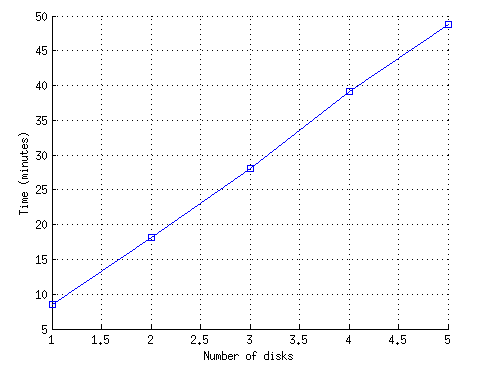
\includegraphics[width=0.65\textwidth]{logic1}
\end{center}
  \caption{Time results for complete erasure by first strategy}
  \label{fig:logic1}
\end{figure}

\newpage
Table \ref{tbl:tbl_logic2} presents the results, which we got during testing the complete erasure with the second strategy.

\begin{table}[h!]
  \caption{Results for complete erasure by second strategy}
  \begin{center}
  \begin{tabularx}{\textwidth}{|p{0.1\linewidth}|p{0.2\linewidth}|X|X|X|X|}
    \hline
    Disks & Capacity & Time & Average time/disk & Average speed
    \\ \hline
    1 & 18.2 GB & 10 min 54 sec & 10 min 54 sec & 27.8 MB/s \\ \hline    
    2 & 36.4 GB & 20 min 42 sec & 10 min 21 sec & 29.3 MB/s \\ \hline
    3 & 54.6 GB & 30 min 41 sec & 10 min 13 sec & 29.6 MB/s \\ \hline
    4 & 72.8 GB & 40 min 25 sec & 10 min 6 sec  & 30.0 MB/s \\ \hline
    5 & 91 GB   & 50 min 10 sec & 10 min 2 sec  & 30.2 MB/s \\ \hline
  \end{tabularx}
  \label{tbl:tbl_logic2}
  \end{center}
\end{table}
Figure \ref{fig:logic2} presents the results from the Table \ref{tbl:tbl_logic2} more clearly.
\begin{figure}[h!]
\begin{center}
  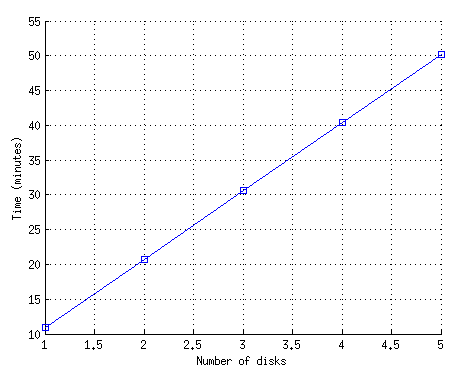
\includegraphics[width=0.65\textwidth]{logic2}
\end{center}
  \caption{Time results for complete erasure by second strategy}
  \label{fig:logic2}
\end{figure}

From these results we can notice that the second strategy works slower than the first one, which is obvious because it needs to change the devices quite often. However, if we compare the Figures \ref{tbl:tbl_logic1} and \ref{fig:logic2} we can see that the difference is only about 1 minute, which is insignificant value in comparison with time for complete erasure of 5 disks, which takes around 50 minutes. 

Table \ref{tbl:tbl_logic3} presents the results, which we got during testing the complete erasure with the third strategy.
\begin{table}[h!]
  \caption{Results for complete erasure by third strategy}
  \begin{center}
  \begin{tabularx}{\textwidth}{|p{0.1\linewidth}|p{0.2\linewidth}|X|X|X|X|}
    \hline
    Disks & Capacity & Time & Average time/disk & Average speed
    \\ \hline
    1  & 18.2 GB  & 6 min 5 sec   & 6 min 5 sec  & 49.8  MB/s \\ \hline    
    2  & 36.4 GB  & 8 min 29 sec  & 4 min 15 sec & 71.5  MB/s \\ \hline
    3  & 54.6 GB  & 9 min 45 sec  & 3 min 15 sec & 93.3  MB/s \\ \hline
    4  & 72.8 GB  & 10 min 57 sec & 2 min 44 sec & 111.2 MB/s \\ \hline
    5  & 91 GB    & 10 min 57 sec & 2 min 11 sec & 138.5 MB/s \\ \hline
    6  & 109.2 GB & 10 min 57 sec & 1 min 50 sec & 166.2 MB/s \\ \hline    
    7  & 127.4 GB & 10 min 57 sec & 1 min 34 sec & 194.0 MB/s \\ \hline
    8  & 145.6 GB & 10 min 57 sec & 1 min 22 sec & 221.7 MB/s \\ \hline
    9  & 163.8 GB & 10 min 58 sec & 1 min 13 sec & 249.0 MB/s \\ \hline
    10 & 182 GB   & 10 min 57 sec & 1 min 6 sec  & 277.1 MB/s \\ \hline    
    11 & 200.2 GB & 11 min 0 sec  & 1 min 0 sec  & 303.4 MB/s \\ \hline    
    12 & 218.4 GB & 11 min 0 sec  & 55 sec       & 331.0 MB/s \\ \hline
    13 & 236.6 GB & 13 min 26 sec & 1 min 2 sec  & 293.6 MB/s \\ \hline
    14 & 254.8 GB & 13 min 28 sec & 58 sec       & 315.5 MB/s \\ \hline
  \end{tabularx}
  \label{tbl:tbl_logic3}
  \end{center}
\end{table}

\newpage
Figure \ref{fig:logic3} presents the results from the Table \ref{tbl:tbl_logic3} more clearly.

\begin{figure}[h!]
\begin{center}
  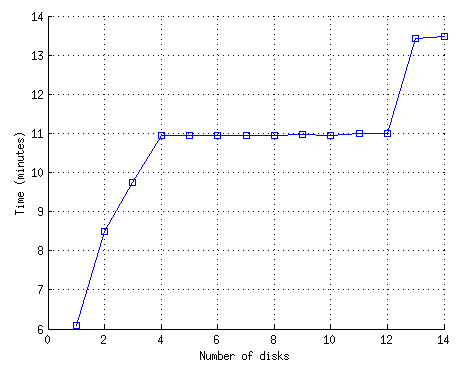
\includegraphics[width=0.65\textwidth]{logic3}
\end{center}
  \caption{Time results for complete erasure by third strategy}
  \label{fig:logic3}
\end{figure}

From the Figure \ref{fig:logic3} we can see that for disks from 4 to 12 the time of complete erasure is constant. Third strategy sends the commands parallel to several disks. That means if there is one slow disk in the task, the whole time of the erasure will be slow. Therefore, we decided to calculate the time of the erasure for single disk.

\newpage
During testing the erasure of single disks with third strategy we got the results presented in the Table \ref{tbl:tbl_logic3_2}. Moreover, in the Table \ref{tbl:tbl_logic3_2} we present the time of erasure for single disk during complete erasure. 

\begin{table}[h!]
  \caption{Results for erasure of single disks by third strategy}
  \begin{center}
  \begin{tabularx}{\textwidth}{|p{0.1\linewidth}|p{0.2\linewidth}|X|X|X}
    \hline
    Disks & Capacity & Time & Time during complete erasure 
    \\ \hline
    1  & 18.2 GB  & 6 min 5 sec   & 6 min 5 sec    \\ \hline    
    2  & 36.4 GB  & 9 min 39 sec  & 10 min 59 sec  \\ \hline
    3  & 54.6 GB  & 9 min 44 sec  & 9 min 43 sec   \\ \hline
    4  & 72.8 GB  & 10 min 57 sec & 10 min 59 sec  \\ \hline
    5  & 91 GB    & 10 min 55 sec & 10 min 53 sec  \\ \hline
    6  & 109.2 GB & 9 min 42 sec  & 9 min 42 sec   \\ \hline    
    7  & 127.4 GB & 6 min 37 sec  & 6 min 37 sec   \\ \hline
    8  & 145.6 GB & 8 min 29 sec  & 8 min 29 sec   \\ \hline
    9  & 163.8 GB & 6 min 38 sec  & 6 min 37 sec   \\ \hline
    10 & 182 GB   & 6 min 5 sec   & 6 min 5 sec    \\ \hline    
    11 & 200.2 GB & 10 min 13 sec & 10 min 12 sec  \\ \hline    
    12 & 218.4 GB & 9 min 51 sec  & 10 min 31 sec  \\ \hline
    13 & 236.6 GB & 9 min 55 sec  & 9 min 55 sec   \\ \hline
    14 & 254.8 GB & 6 min 6 sec   & 6 min 5 sec    \\ \hline
  \end{tabularx}
  \label{tbl:tbl_logic3_2}
  \end{center}
\end{table}

\newpage
Figure \ref{fig:compare_logic3} presents the results from the Table \ref{tbl:tbl_logic3_2} more clearly.
\begin{figure}[h!]
\begin{center}
  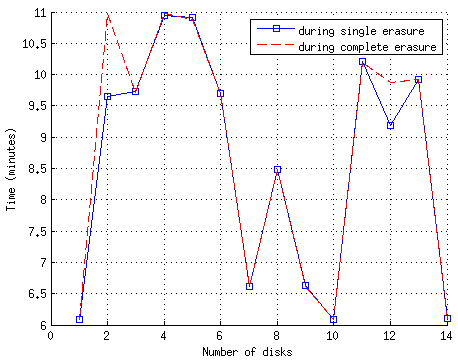
\includegraphics[width=0.65\textwidth]{compare_logic3}
\end{center}
  \caption{Time results for complete erasure by third strategy}
  \label{fig:compare_logic3}
\end{figure}

The third strategy works without any problems, but the results of several disks are quite different, which gives an idea that there are some other parameters of software or hardware, which influence on the speed of the erasure. We can see from the Figures \ref{fig:logic1} and \ref{fig:logic2} that the time of first and second strategies is increasing linearly. We could not say the same about the third strategy because the disks have different speed or some other parameters affect on the maximum speed of the disk. Figure \ref{fig:compare_logic3} shows that the difference is very low between the times of erasure for single disk and for single disk during complete erasure. That means that the bus is not a bottleneck in the situation, when we send WRITE SAME 10 commands parallel to 14 disks, which are connected to the controller. Thus, only speed of the disks is a limiting factor.


By replacing disks 4, 5 and 11 we got different results for the erasure of single disks during complete erasure, which are shown on the Figure \ref{fig:better_res_WS}.
\begin{figure}[h!]
\begin{center}
  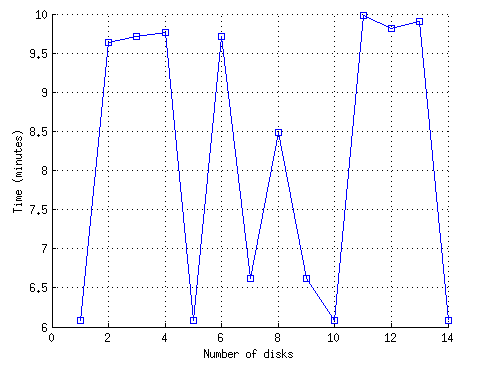
\includegraphics[width=0.65\textwidth]{better_res_WS}
\end{center}
  \caption{Time results for single erasure by third strategy}
  \label{fig:better_res_WS}
\end{figure}

The results from the Figure \ref{fig:better_res_WS} proves the fact that only the disk speed is the limiting factor with the WRITE SAME 10 command. We replaced 3 slow disks and the results show that the time of complete erasure decreased from 11 to 10 minutes. However, it is still strange that the difference of the time of erasure for several disks can be even 4 minutes, which is almost half time of the complete erasure, but the disk parameters are completely the same.



\newpage
\section{Results with WRITE 10 command}
During the research with WRITE SAME 10 command we understood that parallel strategy works pretty well with HP smart Array 642 controller that is why we decided to focus our experiments with WRITE 10 command only on the third strategy. We realized several tests with transfer length 256 which Blancco software uses by default. Table \ref{tbl:tbl_write_10_01} presents the results, which we got during testing the complete erasure with the third strategy.
\begin{table}[h!]
  \caption{Results for erasure of single disks by third strategy}
  \begin{center}
  \begin{tabularx}{\textwidth}{|p{0.1\linewidth}|p{0.2\linewidth}|X|X|X}
    \hline
    Disks & Capacity & Time & Time during complete erasure 
    \\ \hline
    1  & 18.2 GB  & 19 min 52 sec  & 53 min 43 sec (-3)\\ \hline    
    2  & 36.4 GB  & 23 min 24 sec  & 45 min 6 sec  (+4)  \\ \hline
    3  & 54.6 GB  & 23 min 28 sec  & 49 min 25 sec (+3) \\ \hline
    4  & 72.8 GB  & 24 min 43 sec  & 54 min 15 sec (0) \\ \hline
    5  & 91 GB    & 24 min 38 sec  & 57 min 39 sec (-1) \\ \hline
    6  & 109.2 GB & 23 min 28 sec  & 60 min 19 sec (+3) \\ \hline    
    7  & 127.4 GB & 20 min 27 sec  & 54 min 27 sec (+2) \\ \hline
    8  & 145.6 GB & 22 min 15 sec  & 57 min 47 sec (-3) \\ \hline
    9  & 163.8 GB & 20 min 24 sec  & 42 min 40 sec (+2) \\ \hline
    10 & 182 GB   & 19 min 50 sec  & 50 min 37 sec (-5)\\ \hline    
    11 & 200.2 GB & 24 min 1 sec   & 33 min 0 sec  (-5)\\ \hline    
    12 & 218.4 GB & 23 min 32 sec  & 35 min 10 sec (+1)\\ \hline
    13 & 236.6 GB & 23 min 39 sec  & 38 min 14 sec (-6)\\ \hline
    14 & 254.8 GB & 19 min 51 sec  & 52 min 40 sec (-5)\\ \hline
  \end{tabularx}
  \label{tbl:tbl_write_10_01}
  \end{center}
\end{table}

\newpage
Table \ref{tbl:tbl_write_10_01} presents the time results of the erasure of 14 disks with the transfer length 256. The third column shows how much time we need to spend for erasure one single 18.2 GB disk. The forth column consists of the results of time which we need to wait for the erasure of single disk during the parallel erasure of 14 disks. That means that, for example, for disk 13 we need to spend 23 min 39 sec when we erase it separately, but if we erase 14 disks together the erasure of disk 13 will take 38 min 14 sec. Figure \ref{fig:compare_write_10_14disks} presents the results from the Table \ref{tbl:tbl_write_10_01} more clearly.

\begin{figure}[h!]
\begin{center}
  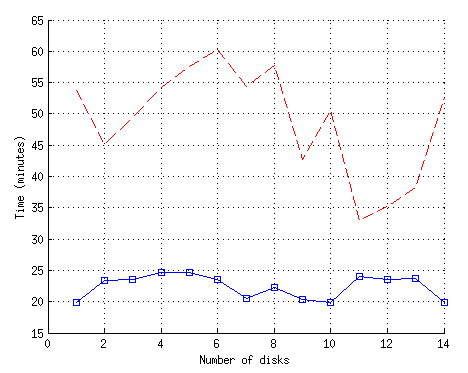
\includegraphics[width=0.65\textwidth]{compare_write_10_14disks}
\end{center}
  \caption{Results for erasure of single disks by third strategy with transfer length 256}
  \label{fig:compare_write_10_14disks}
\end{figure}

The testing results do not depend on the application running and the erasure time is not divided randomly to different disks. Table \ref{tbl:tbl_write_10_01} proved this fact by results from the same test running several times, which gave the whole difference with -13 seconds for erasure of 14 disks by WRITE 10 command. That means that 13 seconds will take only 0.01 of whole erasure process of the fastest disk. That is why we will ignore this difference. 

From the Figure \ref{fig:compare_write_10_14disks} we also can notice how big is the time difference for single erasure if we decide to erase 14 disks together using WRITE 10 command. The lower curve shows us that for erasure one of these 14 disks we need from 20 to 25 minutes. However, if we launch the application together with 14 disks, for the disk 2 it will take 45 minutes, but for disk 10 already 50 minutes. Anyway, the complete erasure takes a bit more than 60 minutes, which is just 3 times bigger than single erasure of the fastest disk. 

The Figure \ref{fig:aver_compl_6-14} presents the graphics of erasure times depending on the amount of disks with the transfer length 256. 

\begin{figure}[h!]
\begin{center}
  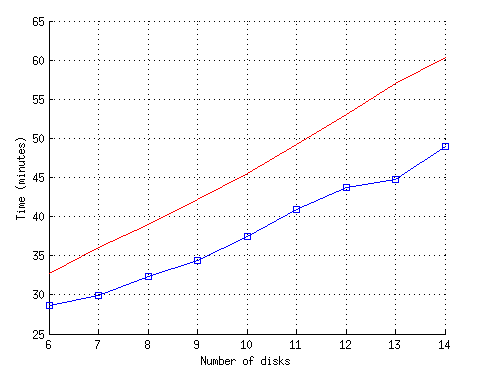
\includegraphics[width=0.65\textwidth]{aver_compl_6-14}
\end{center}
  \caption{Time results for the complete erasure depending on the amount of disks}
  \label{fig:aver_compl_6-14}
\end{figure}

The upper curve of the Figure \ref{fig:aver_compl_6-14} shows the time results of the complete erasure. We can see that the result for the complete erasure of 14 disks is equal to the result from the Figure \ref{fig:compare_write_10_14disks}. The lower curve shows the average time results for single erasure during complete erasure. That means that when we divide the sum of the values from the forth column of the Table \ref{tbl:tbl_write_10_01} by 14, we will get the last value of the curve for average time from the Figure \ref{fig:aver_compl_6-14}. From the Figure \ref{fig:aver_compl_6-14} we can make a conclusion that addition of 1 disk gives us addition of 3 minutes to the complete erasure.

We can notice from the Figure \ref{fig:compare_logic3} that during complete erasure by WRITE SAME 10 command disks 2, 4 and 5 showed the worst time. In the same time the Figure \ref{fig:compare_write_10_14disks} presents that during complete erasure by WRITE 10 command disks 6 and 8 showed the worst time. That gives an idea that there are some other parameters which also influence on the time of erasure. It is possible that the controller decides which command goes first and to which device. Thus, we could not influence on that fact. We decided to replace disks 4, 5 and 11 and check how it will change the situation. The Figure \ref{fig:comp_disk_repl_W10} shows these results. 

\begin{figure}[h!]
\begin{center}
  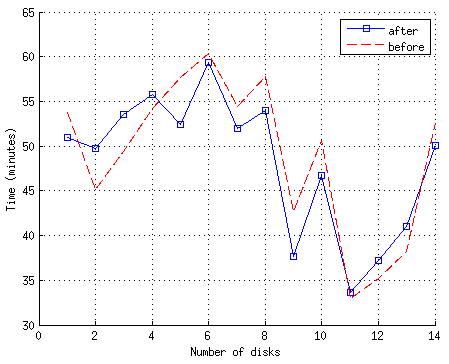
\includegraphics[width=0.65\textwidth]{comp_disk_repl_W10}
\end{center}
  \caption{Results after replacement of the disks 4, 5 and 11.}
  \label{fig:comp_disk_repl_W10}
\end{figure}

From these results we can conclude that time for complete erasure decreased for 1 minute and the same disks show the maximum and minimum times. However, it is strange that during single erasure by WRITE 10 command disks 1 and 14 were the fastest and during complete erasure their results are closed to very slow ones.

We discussed before that transfer length is one the most important parameters during the erasure by WRITE 10 command. Furthermore, we can influence on it. Figure \ref{fig:diff_transfer_length_diskF} presents the time results for the erasure of disk 1 depending on the different transfer length.

\begin{figure}[h!]
\begin{center}
  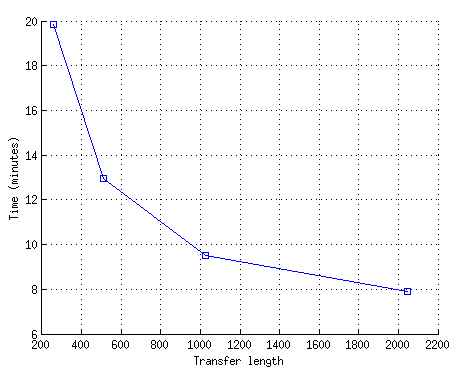
\includegraphics[width=0.65\textwidth]{diff_transfer_length_diskF}
\end{center}
  \caption{Time results for the disk 1}
  \label{fig:diff_transfer_length_diskF}
\end{figure}

The Figure \ref{fig:diff_transfer_length_diskF} shows that 2048 is the optimal value for 1 disk. If we take the value, for example, 4096, which is bigger that 2048, we come to the situation when we get errors from the WRITE 10 command. It happens because the limit of 2 MB is exceeded and the driver cannot handle so big amount of information. The Figure \ref{fig:diff_transfer_length_diskF} shows that  we need for erasure of disk 1 with transfer length 2048 only 8 minutes, which is 12 minutes faster than the erasure with transfer length 256. This result proves the fact that we can influence on the speed erasure by varying the transfer length. Thus, we can achieve faster erasure by finding the optimal transfer lengths depending on the amount of disks. Our suggested load balancing system will help with solving this problem.

The Figure \ref{fig:diff_length_14disks} shows the results of testing different transfer length during erasure of 14 disks in the same time.

\begin{figure}[h!]
\begin{center}
  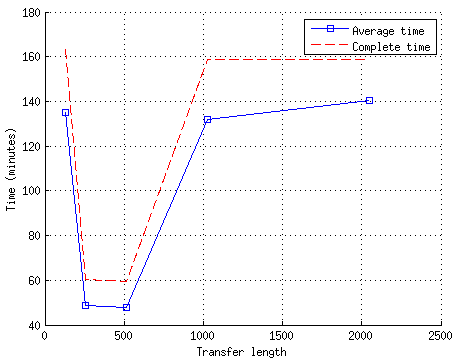
\includegraphics[width=0.65\textwidth]{diff_length_14disks}
\end{center}
  \caption{Time results for average erasure and complete erasure depending on the transfer length}
  \label{fig:diff_length_14disks}
\end{figure}

To summarize the results from the Figure \ref{fig:diff_length_14disks} we can say that transfer lengths 512 and 256 give almost the same results, but the optimal value for 14 disks is 512, which is easier to see from Figure \ref{fig:comp_256_512length}. 

Figure \ref{fig:comp_256_512length} presents the time results of complete erasure with transfer length 256 and 512.
\begin{figure}[h!]
\begin{center}
  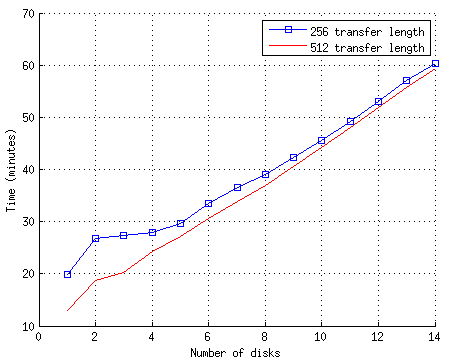
\includegraphics[width=0.65\textwidth]{comp_256_512length}
\end{center}
  \caption{Results for complete erasure with transfer lengths 256 and 512 depending on the amount of disks}
  \label{fig:comp_256_512length}
\end{figure}

\newpage
Figure \ref{fig:comp_256_best_length} presents the time results of theoretical optimal complete erasure in comparison with the results with transfer length 256.

\begin{figure}[h!]
\begin{center}
  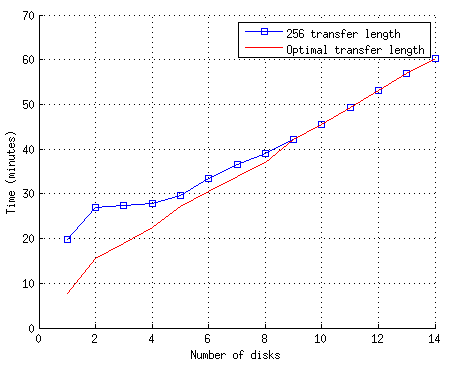
\includegraphics[width=0.65\textwidth]{comp_256_best_length}
\end{center}
  \caption{Results for theoretical optimal erasure}
  \label{fig:comp_256_best_length}
\end{figure}

These graphics show the difference between the results of our suggested load balancing system and Blancco software at the moment. Load balancing system applies the Formula \ref{eq:optimal_length} to calculate the optimal transfer length. Thus, if we apply only our theoretical calculations the Figure \ref{fig:comp_256_best_length} shows the results of time improvement.  For the disks 1-8 we took another transfer length, which improves the time of erasure. For disk 1 and 2 the transfer length was 2048, for disk 3 and 4 - 1024, and for disks from 5 to 8 - 512.

%We can see from the Figure \ref{fig:comp_256_best_length} that disks 1-8 have the differences of the results.

Moreover, using our practical results we can suggest to apply the results from the Figure \ref{fig:comp_256_best2_length}, which improves the Blancco software for any amount of disks. The difference between theoretical optimal erasure and practical optimal erasure is another transfer length for disks 9-14. In practise, when we took the transfer length 512 we got better results in comparison with theoretical optimal erasure. These results shows that the optimal transfer length, which was calculated by testing and load balancing system, makes the erasure faster for WRITE 10 command from disk 1 to disk 14.

\begin{figure}[h!]
\begin{center}
  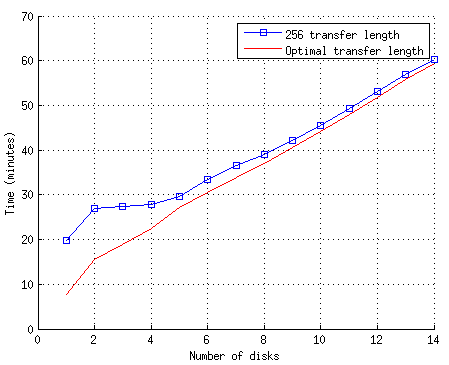
\includegraphics[width=0.65\textwidth]{comp_256_best2_length}
\end{center}
  \caption{Results for practical optimal erasure}
  \label{fig:comp_256_best2_length}
\end{figure}




